%!TEX root = report.tex
\chapter{Evaluation}
\label{ch:evaluation}
\par This chapter documented the evaluations of the API endpoints. We first quantified the accuracy of the \acrshort{tfl} Live Bus Arrivals API. We then tested the correctness and performance of our data service API endpoints. Lastly, we evaluated the accuracy of the generated bus timetables.

\section{Accuracy of TfL Live Bus Arrivals API}
\label{sec:tfl_stream_accuracy}
\par The Tfl Live Bus Arrivals API updates the bus arrival times every 30 seconds. This means that the accuracy of the bus arrival predictions for the current stop will improve gradually as the bus approaches the stop. This is because any error in earlier predictions would be incrementally corrected at every update as the location of the bus gets refreshed.

\subsection{Test for Accuracy}
\par We evaluated the accuracy of these predictions by the following steps:

\begin{itemize}
  \item We took a snapshot of all the bus arrivals predictions for the next 30 minutes at a given recorded time (2015-06-04 11:24:37).
  \item We grouped these prediciton entries by the difference between the predicted arrival time and the recorded time at a 5-minute interval. For example, the predictions for the buses arriving in the next 5 minutes, next 5 to 10 minutes, and next 10 to 15 minutes, etc. We added an additional group for the next 0 - 3 minutes for reference.
  \item After 3 hours, we compared each arrival prediction entry in the snapshot table against the actual arrival data we stored for generating the current timetable. The difference between the predicted and the actual arrival time gives an indication of the prediction accuracy. We stored this difference as the delta value. A negative delta indicates the bus came later than the predicted time.
  \item We calcuated the mean delta for each group, and created Table \ref{table:countdown_evaluation}.
\end{itemize}

\begin{table}
\centering
\begin{tabular}{@{}lr@{}} \toprule
TfL Live Bus Arrivals for & Mean Delta (Seconds) \\ \midrule
next 0 - 3 mintues & -34.8112 \\
next 0 - 5 mintues & -45.4951 \\
next 5 - 10 mintues & -97.2584 \\
next 10 - 15 mintues & -134.3606 \\
next 15 - 20 mintues & -169.5990 \\
next 20 - 25 mintues & -174.7177 \\
next 25 - 30 minutes & -166.1368 \\
\bottomrule
\end{tabular}
\caption{Live Bus Arrivals API Accuracy - A negative delta indicates the bus came later than the predicted time}
\label{table:countdown_evaluation}
\end{table}

\subsection{Test Result}
\par Table \ref{table:countdown_evaluation} shows that buses usually came later than the predictions provided by the TfL Live Bus Arrivals API. For the buses that were predicted to arrive in the next 5 minutes, they usually came less than one minute later than the predicted arrival time. The distribution of the difference between the \acrshort{tfl} Live Bus Arrivals API and the actual bus arrival times is shown in Figure \ref{fig:countdown}. We can see that the predictions for the next 5 mintes have smaller errors compared to the restas the peak is much higher near zero errors. We took this finding into consideration when testing the accuracy of our current and historical timetable by only choosing buses that are due within the next 5 minutes as tracking targets.

\begin{figure}
\centering
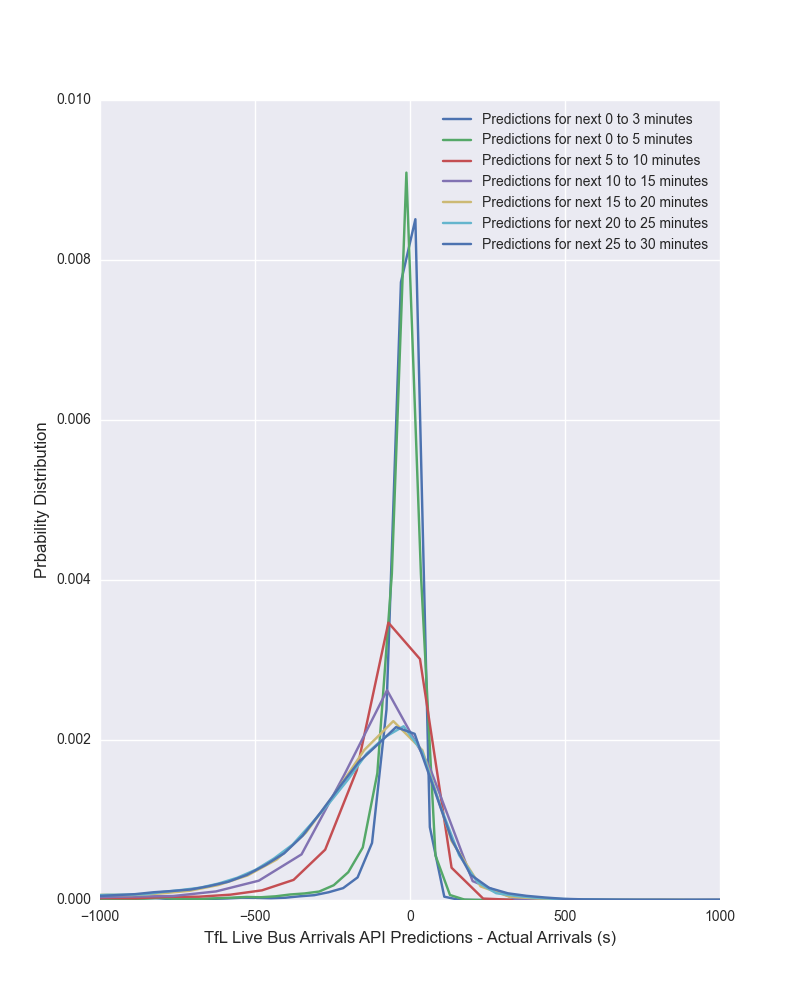
\includegraphics[width=\textwidth]{figures/countdown.png}
\caption{\label{fig:countdown} Delta Distribution of TfL Live Bus Arrivals API}
\end{figure}


\section{Correctness and Performance of the API}
\subsection{Tool}
\par We used \textit{siege}\cite{siege} to conduct the load test of our API endpoints. Our aim was to test the number requests the server could handle reliably at one time, and the response time it took.

\par \textit{Siege} takes in the number of users, the delay time between each page load, the test running time, and the list of URLs to send requests to as parameters. It then simulates the user behaviours to fire requests to the list of given URLs. At the end of the test, \textit{Siege} generates a report for the test, including metrics such as the transaction rate, and the response time of the target URLs.

\subsection{Preparation}
\par We generated a list of API URLs with random parameters for testing. We then ran the siege tests by fixing the test running time to be 1 minute, with 1 second of delay between each page load.

\subsection{Test for Correctness}
\par We first tested for the correctness of our API endpoints. This involves firing requests with random day of the week and hour of day, route, run, and starting bus stop code to check whether the server can return a response correctly.

\par At this stage, we found some specific URLs that resulted in a 500 error code, and debugged the backend code to return correct results. For example, this happened when we requested for a reference travel time for a bus route at an hour out of its operating time. As there was no corresponding entry in the databases, we fixed the code by returning an empty list by default.

\par After we received 200 status code for all requests in a few test runs consistently, we proceeded to perform the load tests by fixing the day of the week and hour of the day to be the current values when the test was run.

\subsection{Load Test for Performance}
\par We carried out the siege test with various number of concurrent users ranging from 50 to 500, on a list of URLs with randomly selected parameters. We collected the test results and plotted the figures for availability, response time, and transaction rates \cite{siege_manual}. The metrics are defined as:

\begin{itemize}
  \item \texttt{Response time} is the average time it took to respond to each simulated user’s requests.

  \item \texttt{Transaction rate} is the average number of transactions the server was able to handle per second, in a nutshell: transactions divided by elapsed time.

  \item \texttt{Successful transactions} is the number of times the server returned a code less than 400. Accordingly, redirects are considered successful transactions.

  \item \texttt{Avalability} is the percentage of successful transactions over the total number of server hits.
\end{itemize}


\subsubsection{Historical \& Current Timetables API Performance}

\par Figure \ref{fig:siege_pre_api_availability} shows that the \texttt{availability} drops below 100\% when there were more than 100 users accessing the API simultaneously. We used this as a benchmark for the number of uses the current server can reliably handle. Figure \ref{fig:siege_pre_api_response_time} shows that the average \texttt{response time} for 100 users is approximately 15 seconds, and increases as the number of users increases. Figure \ref{fig:siege_pre_api_transfer_rate} shows that the \texttt{transaction rate} for 100 users is about 5.5 transactions per second.

\textbf{Cause of slow response}. The slow response time was probably due to the number of databases query required to form a response. One databases query was needed for every pair of neighbouring stops in the downstream stop sequence to retrieve the timetable entry. One potential approach to reduce the number of databases query is to produce the bus journey timetables by route. In this case, only one query would be sufficient for each request. The tradeoff is that the tables will be larger as there will be multiple entries for the same pair of neighbouring stops on different routes. We discussed other potential improvement for performance in Chapter \ref{ch:future_work}.

\begin{figure}
\centering
\includegraphics[width=0.8\textwidth]{figures/siege_predictions_api_availability_against_users.pdf}
\caption{\label{fig:siege_pre_api_availability} Historical \& Current Timetables API Availability against no. of simultaneous users}
\end{figure}

\begin{figure}
\centering
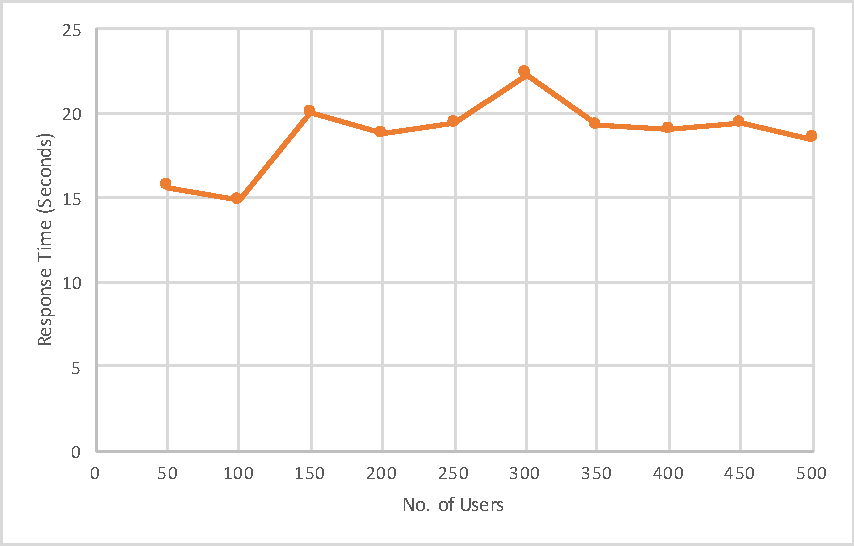
\includegraphics[width=0.8\textwidth]{figures/siege_predictions_api_response_time_against_users.pdf}
\caption{\label{fig:siege_pre_api_response_time} Historical \& Current Timetables API Response Time (seconds) against no. of simultaneous users}
\end{figure}

\begin{figure}
\centering
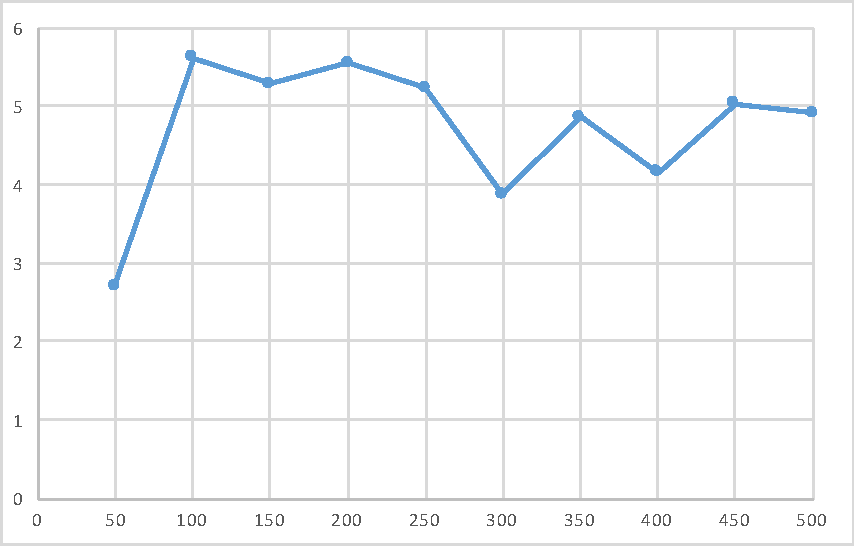
\includegraphics[width=0.8\textwidth]{figures/siege_predictions_api_transfer_rate_against_users.pdf}
\caption{\label{fig:siege_pre_api_transfer_rate} Historical \& Current Timetables API Transaction Rate against no. of simultaneous users}
\end{figure}

\subsubsection{Reference Timetable API Performance}
\par Figure \ref{fig:siege_tfl_api_availability} shows that the \texttt{availability} drops below 100\% when there were more than 150 users sending requests to the Reference Timetable API endpoint concurrently. The average \texttt{response time} for 150 users is about 4.5 seconds (Figure \ref{fig:siege_tfl_api_response_time}), and the \texttt{transaction rate} is approximately 27 transactions per second (Figure \ref{fig:siege_tfl_api_transfer_rate}). The performance of this endpoint is better as every request involves only one databases query.

\begin{figure}
\centering
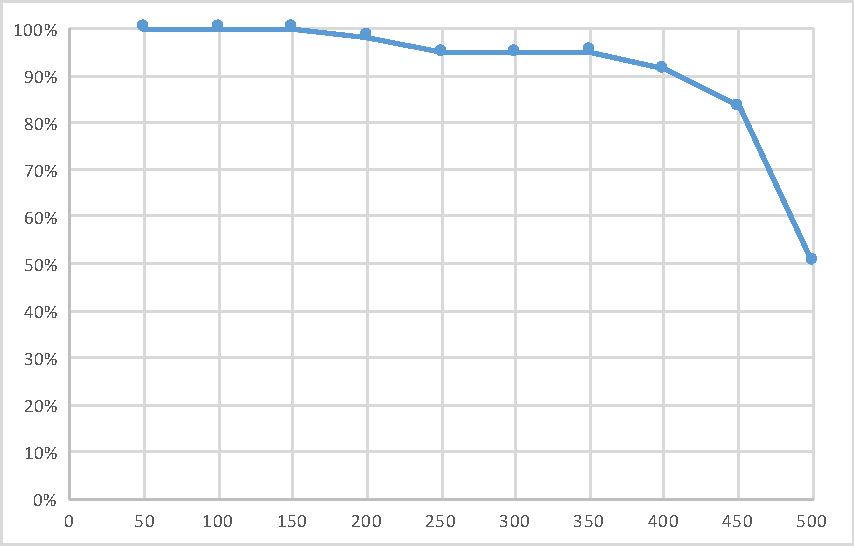
\includegraphics[width=0.8\textwidth]{figures/siege_tfl_api_availability_against_users.pdf}
\caption{\label{fig:siege_tfl_api_availability} Reference Timetables API Availability against no. of simultaneous users}
\end{figure}

\begin{figure}
\centering
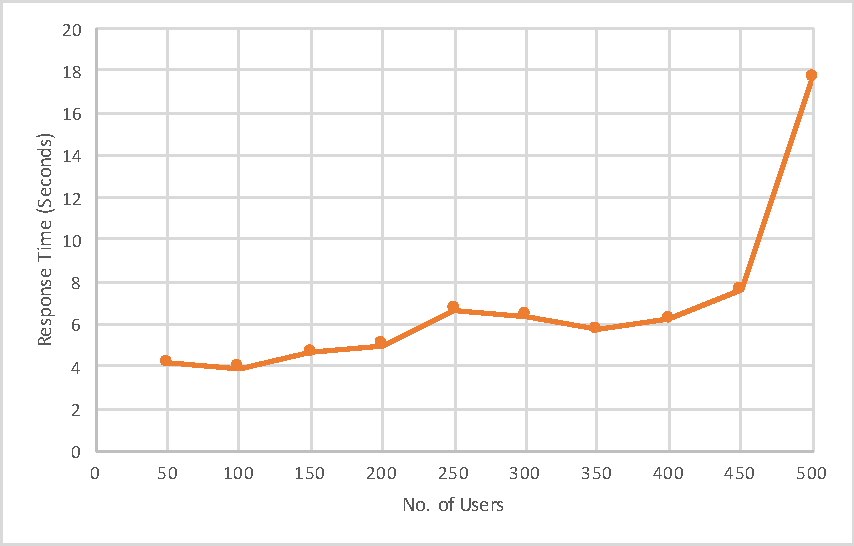
\includegraphics[width=0.8\textwidth]{figures/siege_tfl_response_time_against_users.pdf}
\caption{\label{fig:siege_tfl_api_response_time} Reference Timetables API Response Time (seconds) against no. of simultaneous users}
\end{figure}

\begin{figure}
\centering
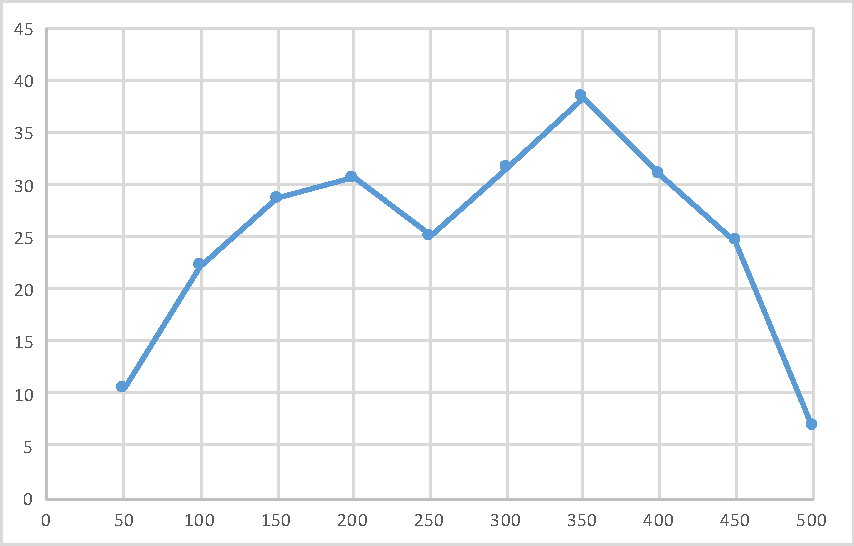
\includegraphics[width=0.8\textwidth]{figures/siege_tfl_transfer_rate_against_users.pdf}
\caption{\label{fig:siege_tfl_api_transfer_rate} Reference Timetables API Transaction Rate against no. of simultaneous users}
\end{figure}

\section{Accuracy of Predictions}
\label{sec:prediction_accuracy}
\par To evaluate the accuracy of the bus journey time predictions, we ran tests to compare the actual bus travel times with the historical, current, and reference timetables respectively. We achieved this by first saving the predicted bus journey times from the two endpoints for a given vehicle. We then searched the databases for the actual arrival time records for the vehicle at each downstream stops. For each test case, we ran through the steps below:

\begin{enumerate}
  \item \textbf{Saving predicted bus journey times}:
  \begin{enumerate}
    \item Fix day of the week and hour of the day to be the current value when the test was run.
    \item Generate random parameters for the route, bus direction, current starting stop on the route.
    \item Generate the URL and send request to obtain the next vehicle arrival time for the given route at the given stop from the \acrshort{tfl} Live Bus Arrivals API. If the next vehicle is due in more than 5 minutes later, repeat steps 1(a) and 1(b) until there is a case with a next vehicle due within 5 minutes.
    \item  Generate the historical \& current, and reference timetable URLs with the same set of parameters.
    \item Send requests to the above URLs to obtain a snapshot of the reference, historical and current bus travel timetables for the given route at the given hour of the given day.
    \item Save the responses for comparison with the actual arrivals data later.
  \end{enumerate}
  \item Wait for a few hours to allow the target vehicle to travel to the terminal. The arrival times for the target vehicle at each downstream stop should have been recorded in the database.
  \item \textbf{Comparing predictions to actual travel times}:
  \begin{enumerate}
    \item For each target vehicle, retrieve its actual arrival times at each downstream stop from the given starting stop.
    \item Compute the actual bus travel time in seconds between the given starting stop and each downstream stop.
    \item Compare the actual bus travel times with the reference, historical, and current bus travel times for each pair of the starting stop and ending stop respectively.
  \end{enumerate}
\end{enumerate}

\par We collected 154 test cases throughout the day on 12 June 2015. Each test case consists of a list of travel times from the starting stop to each downstream stop. There were 3362 pair of stops in total. We ploted the probability density graph to compare the reference, historical and current bus travel times with the actual bus travel times.
\todo[inline]{insert graph}

\par We found that the individual predictions do not give satisfactory accuracy.



